\section*{Problem Statement}
The objective of this problem is to demonstrate the convergence of the estimated value of $\pi$ using the Monte Carlo simulation method, with an increasing number of iterations.

\section*{Methodology}
The Monte Carlo method relies on generating random points inside a unit square $[0,1] \times [0,1]$ and determining the proportion of points that fall inside the quarter unit circle defined by $x^2 + y^2 \leq 1$. Since the area of this quarter circle is $\pi/4$, the ratio can be used to estimate $\pi$.

\subsection*{Pseudo-code}
\begin{enumerate}
  \item Initialize counters for points inside and outside the circle.
  \item For each iteration:
  \begin{enumerate}
    \item Sample random $x, y \in [0,1]$.
    \item Compute distance $d = \sqrt{x^2 + y^2}$.
    \item If $d \leq 1$, classify point as inside; otherwise classify as outside.
  \end{enumerate}
  \item Estimate $\pi$ as:
  \[
    \pi \approx 4 \times \frac{\text{number of points inside}}{\text{total number of points}}
  \]
  \item Repeat with increasing iterations (e.g., $64, 640, 6400, 64000$).
  \item Record and plot the results.
\end{enumerate}

\section*{Results}
The following figures illustrate the distribution of points for different iteration counts, along with the corresponding approximation of $\pi$. As the number of iterations increases, the estimate converges towards the true value of $\pi$.

\begin{figure}[h!]
  \centering

    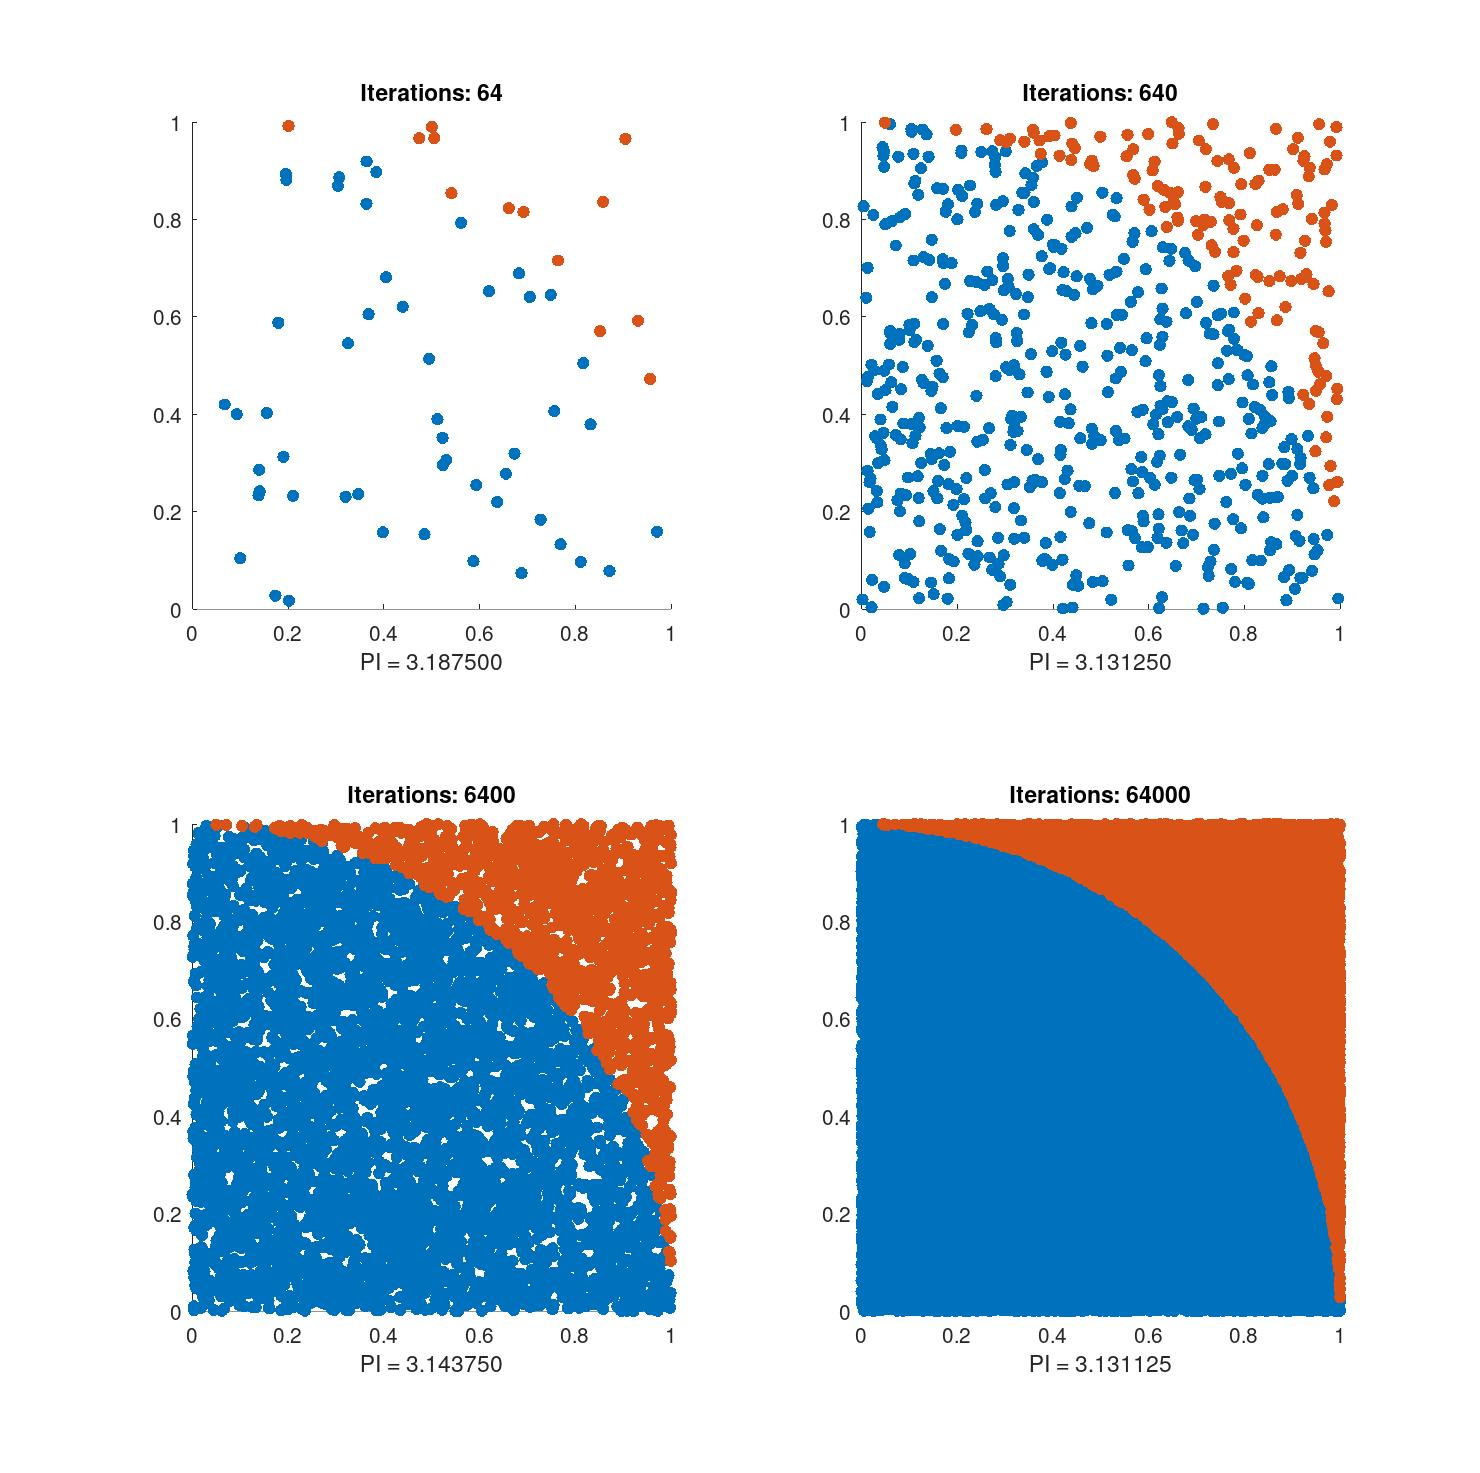
\includegraphics[width=0.75\textwidth]{a1.jpg}
    \caption{Monte Carlo simulation of $\pi$ with increasing iterations.}
\end{figure}

\section*{Conclusion}
The Monte Carlo simulation provides a stochastic method for estimating $\pi$. With a small number of iterations, the estimate is inaccurate, but as the iteration count increases, the estimate converges to the true value of $\pi$.
